\documentclass[12pt,a4paper]{report}
\usepackage[frenchb]{babel}
\usepackage[utf8]{inputenc}
\usepackage[export]{adjustbox}
\usepackage[margin=2cm]{geometry}
\usepackage{verbatim}
\usepackage{amsmath}
\usepackage{amsfonts}
\usepackage{amssymb}
\usepackage{listings}
\usepackage{graphicx}
\usepackage{pgf, tikz}
	\usetikzlibrary{arrows, shapes, positioning}
\usepackage{hyperref}
\hypersetup{%
    pdfborder = {0 0 0}
}
\author{Maugey Rémy - Bernard Jérémi - De Pourquéry Benjamin - Decoudras Hadrien}
\title{Rapport projet compilation}

\usepackage{tikz}

\begin{document}

\begin{titlepage}
  \begin{sffamily}
  \begin{center}

    % Upper part of the page. The '~' is needed because \\
    % only works if a paragraph has started.
    
\includegraphics[scale=0.05]{logo.jpg}~\\[1.5cm]
    % Author and supervisor
    \begin{minipage}{0.43\textwidth}
      \begin{flushleft} \large
		MAUGEY Rémy\\
		De POURQUERY Benjamin\\
		DECOUDRAS Hadrien\\
		BERNARD Jérémi\\		
		
      \end{flushleft}
    \end{minipage}

	\topskip0pt
	\vspace*{\fill}
	\Huge{Rapport de projet technologique}\\
	\Large{Vision stéréoscopique pour robot}\\
	\vspace*{\fill}

	\vfill
    % Bottom of the page
    \begin{small}
 	Licence $3^{\text{ème}}$ année\\
 	\end{small}
    {\large \today}\\

  \end{center}
  \end{sffamily}
\end{titlepage}

\chapter{Introduction}


L'objectif de ce projet est de développer un outil implémenté sur un robot lui permettant de suivre à un mètre une personne grâce à deux caméras.\\\\

Le projet est divisé en deux parties indépendantes, effectuées sur les deux semestres. 
La première partie a pour but de prendre en main les outils utilisés au cours de l'année, à savoir le langage C++ (à travers Qt) et la bibliothèque OpenCV.
Durant cette première partie sera développé un mini programme de traitement d'image. 

La deuxième partie a pour objectif de programmer le robot et d'effectuer des simulations grâce au logiciel Unity. En effet, comme le robot n'est pas forcément accessible aux membres du groupe, il est préférable de faire appel à une simulation pour pouvoir tester les algorithmes n'importe quand.\\\\

Qt est une bibliothèque logicielle d'interface graphique, nous utiliserons cet outil pour développer l'interface du logiciel.\\

OpenCV (Open Computer Vision) est une bibliothèque pincipalement d'algorithmes de traitement d'image et de vidéos. Ici elle sera utilisée pour programmer les fonctions du logiciel en rapport avec les images.\\


%Petite explication de la procédure de comment fonctionne la stereovision ...
\section{Cahier des charges}
Le cahier des charges s'oriente uniquement sur l'objectif du projet, c'est à dire sur la deuxième partie du semestre.
\subsection{Besoins fonctionnels}
	%Identifie une personne
	%Se meut
	%Calcule une distance
	Le logiciel doit prendre en entrée deux images au format \textit{PNG} représentant les images gauche et droite de deux caméras.
	Ces images vont nous permettre de créer une carte de disparité de la scène.\\	
	Cette dernière additionnée aux caractéristiques de la caméra va nous permettre de créer une carte de profondeur. Qui sera ensuite utilisée pour permettre au robot de se déplacer.\\
	Il sera cependant nécessaire d'avoir une carte de profondeur de référence de la personne à suivre à travers une phase d'initialisation. Dans ce cas, la première image prise par le robot permettra de créer la première carte de profondeur qui sera considérée comme la référence. Il faut donc que le robot soit bien placé à un mètre de la personne lors du démarrage et que cette dernière soit la seule dans le cadre des caméras.
\subsection{Besoins non fonctionnels}
	%Robuste aux chagement de luminosité
	%changement de personne
	%chagement d'environnement
	La carte de disparité est fortement liée aux images d'entrée, de ce fait, les changements de luminosité et d'environnement peuvent poser des problèmes à cause notamment de l'utilisation d'une référence, nécessaire pour reconnaître la personne.\\
	Le programme doit donc être robuste à ces différents changements.\\
	Le robot doit être aussi capable de suivre la bonne personne même si une autre personne rentre dans le cadre.
	
\chapter{Théorie et définitions}
%capture des images
%création de la carte de disparité + def 
%création de la carte de profondeur + def et formule
%mouvement du robot

Comme montré dans la figure 2.1.1, le projet se structure autour d'une notion clef : Pour repérer les jambes d'une personne afin de la suivre, une carte de profondeur doit être calculée. Cette carte est créée grâce à une carte de disparité. 

\begin{center}
\begin{tikzpicture}
	\node[draw] (capture) 	at (-4,0) 	{Images};
	\node[draw]	(disp)		at (0,0) 	{Carte de disparité};
	\node[draw] (depth)		at (5,0)	{Carte de profondeur};
	
	\draw[->]	(capture) to (disp);
	\draw[->]	(disp) to (depth);
\end{tikzpicture}\\
Figure 2.1.1 Fil rouge du projet.
\end{center}

\paragraph{Carte de disparité}
Un carte de disparité est une image où chaque pixel correspond au déplacement d'un même point dans deux images différentes. 

\begin{center}
	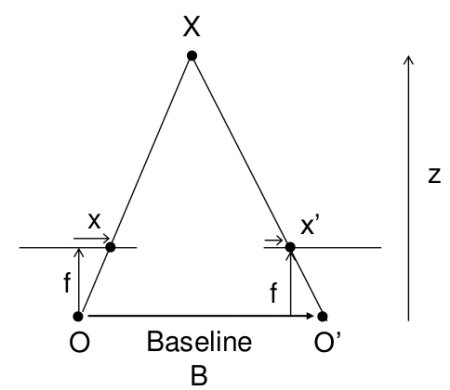
\includegraphics[scale=0.5]{disparity.jpg}\\
	Figure 2.1.2 Schéma du calcul de la carte de disparité.\footnote{Source : \url{http://docs.OpenCV.org/3.0-beta/doc/py_tutorials/py_calib3d/py_depthmap/py_depthmap.html}}\\
\end{center}

Comme représentée dans la figure 2.1.2, la valeur du pixel X représente le déplacement du pixel.
Les deux images sont représentées par O et O' et la longueur en cm entre elles par la baseline B.
\paragraph{Carte de profondeur}
La carte de profondeur est une image où chaque pixel représente la distance entre le robot et le point dans le monde réel. Cette distance est exprimable en mètres.\\
La formule permettant de calculer la carte de profondeur à partir de la carte de disparité est une application du théorème de Thalès.\\

\begin{center}
Figure 2.2.3 Formule de la carte de profondeur.\\

\begin{huge}
$\text{depth} = \frac{\text{baseline} * \text{focal}}{\frac{\text{disp}}{\text{width}} * \text{sensor size}} / \text{reference}$\\
\end{huge}
\end{center}
\paragraph{Légende : }
\begin{small}
\begin{enumerate}
\item[-] baseline : distance entre les centres des deux caméras.\\
\item[-] focal : focal de l'objectif.\\
\item[-] disp : valeur du pixel de la carte de disparité.\\
\item[-] width : largeur de l'image.\\
\item[-] sensor size : taille du capteur.\\
\item[-] référence : distance voulue (dans le cadre de ce projet, en mètres donc 1000).\\
\end{enumerate}
\end{small}

On peut calculer une carte de profondeur en utilisant la formule ci-dessus sur chaque pixel ou bien utiliser une fonction d'OpenCV :  

\begin{lstlisting}{Language=C++}
void reprojectImageTo3D(InputArray disp, 
			OutputArray out, 
			InputArray Q, 
			bool handleMissingValues, 
			int ddepth);
\end{lstlisting}

\paragraph{Problèmes rencontrés}
L'utilisation de la \textit{reprojectImageTo3D} implique de devoir au préalable calibrer les caméras et rectifier les images, étapes longues et non obligatoires car les caméras fournies sont suffisamment fiables. Donc nous avons décidé de ne pas l'utiliser.

\chapter{Implémentation}

\section{Logiciel Qt}
%Partie Qt
Le premier semestre s'est orienté autour du développement d'un petit programme de traitement d'image. Le programme affiche une fenêtre ainsi que plusieurs menus, l'un d'eux permet d'ouvrir un fichier dans l'un des formats supportés par OpenCV.
Le fichier doit nécessairement contenir les deux images juxtaposées pour que notre programme fonctionne. On peut ensuite couper l'image en deux, la flouter grâce à la méthode "blur" d'OpenCV. On peut aussi appliquer à l'image différents algorithmes comme celui de Sobel ou encore celui de Canny tous deux permettent de faire de la détection de contours, présentés sur les figures ci contre.
\begin{center}
\begin{tabular}{cc}
  \vspace{0pt} 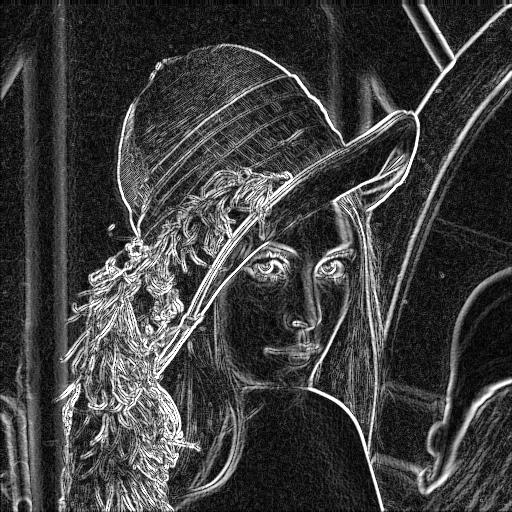
\includegraphics[width=0.49\textwidth]{sobel.jpg} &
  \vspace{0pt} 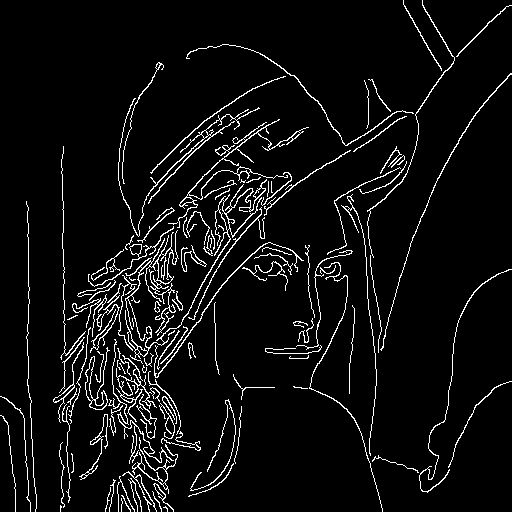
\includegraphics[width=0.49\textwidth]{canny.jpg} \\
    
  Figure 3.1.1 Sobel & Figure 3.1.2 Canny
\end{tabular}
\end{center}

Ces différentes méthodes ont été implémentées dans le but de comprendre le fonctionnement d'OpenCV, ainsi que de développer et de tester une première esquisse des fonctions que nous utiliserons dans le robot.

Il a fallu créer des méthodes de conversion d'images entre les images de Qt et les images de OpenCV. Deux méthodes ont donc été développées : 

\begin{lstlisting}{Language=C++}
cv::Mat ImageTools::imageToMat(QImage const& src);
QImage ImageTools::cvMatToImage(const cv::Mat& inMat);
\end{lstlisting}

Toutes les méthodes en rapport avec le traitement d'image ont été implémentées dans la classe \textit{imagetools}. Au début, nous conservions les images sous forme de QImage ce qui nous obligeait à les convertir à chaque fois que l'on voulait appliquer un filtre. On a fini par réécrire entièrement le programme, où l'on conserve les images sous forme de matrices OpenCV en images membres et la classe \textit{imagetools} sous forme d'un singleton, simplifiant le code.\\
Le logiciel permet aussi de faire de la reconnaissance de formes grâce aux algorithmes de \textit{flann} et de \textit{surf}. Cependant ce dernier n'est pas open source donc la méthode \textit{flann} est implémenté entre \textit{\#define} et n'est pas forcément proposé à l'utilisateur final.\\
Enfin, le logiciel permet de créer une carte de disparité grâce à l'algorithme \textit{stereosgbm} ou à l'algorithme \textit{stereobm}.\\

Cette partie nous a permis de prendre en main le C++ ainsi que la bibliothèque OpenCV.\\

Grâce à ce petit outil, nous avons testé les deux algorithmes permettant de générer des cartes de disparité. Nous avons ainsi retenu \textit{stereosgbm} qui est moins performant mais plus simple à utiliser et crée moins de bruit. Cela nous a permis de choisir des paramètres de \textit{stereosgbm} jugés bons.\\

Le logiciel Qt prend aussi en charge diverses fonctions propres à Qt et non d'OpenCV tel que le redimensionnement des images, grâce à la méthode cropImage() ou encore la possibilité de zoomer dans l'image.

\section{Simulation et test}
%partie Unity
Durant le second semestre, l'objectif était d'implémenter les algorithmes précédents pour les utiliser sur le robot. Le but est de créer une carte de profondeur grâce aux images du robot pour lui permettre de se déplacer en fonction de la position de la personne.\\
Comme nous n'avons pas forcément accès au robot, nous avons décidé de faire une simulation simple sur le logiciel Unity.\\

Unity est un outil qui permet dans sa fonction principale de créer des applications 3D telles que des jeux vidéo. Il permet grâce à une interface de placer des objets dans une scène et une ou plusieurs caméras. Le logiciel inclut aussi une gestion avancée des interactions physiques entre les objets de la scène, le tout très paramétrable grâce aux scripts. Il existe deux langages de script implémentés dans le logiciel, le C\# et le Javascript. Durant ce projet nous avons fait le choix d'utiliser le C\# car l'API est plus complète que celle du JS.
Ce langage de script est à la base un langage de programmation de haut niveau développé par Microsoft dans les années 2000 exclusivement pour la plateforme Windows, mais qui dans ce cas présent est utilisé en temps que langage de script grâce à son implémentation libre Mono. Le C\# a une syntaxe proche du Java. Mais il est quand même plus souple car il prend en charge les systèmes de "namespace" ainsi que la gestion de la surcharge d'opérateurs. Le langage permet même d'utiliser des pointeurs sous forme de blocs "unsafe"\footnote{Gestion des pointeurs en C\# : \url{https://msdn.microsoft.com/en-us/library/y31yhkeb.aspx}} mais son utilisation sous Unity n'est pas convaincante.

	\begin{center}
		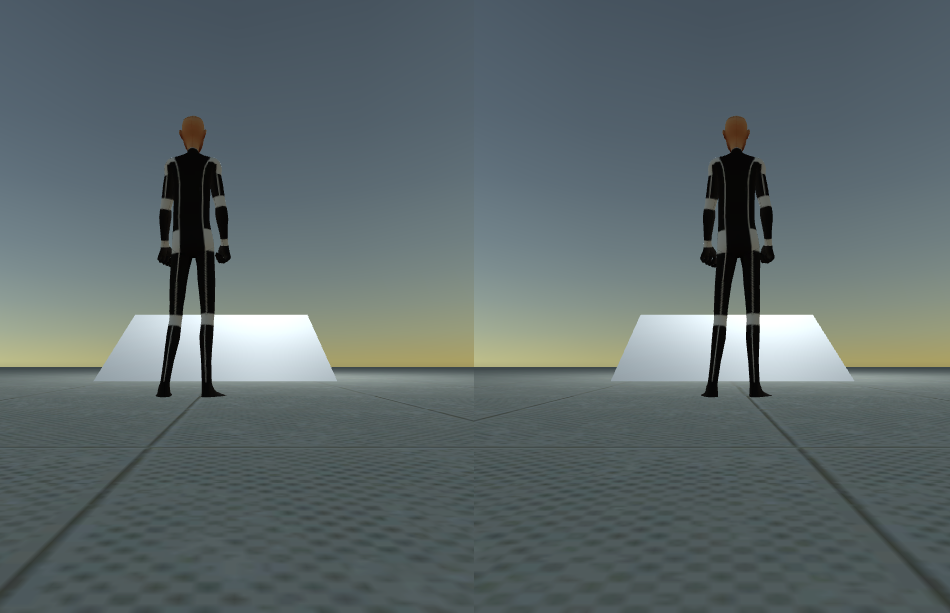
\includegraphics[scale=0.5]{Screenshot_skybox.png}\\
		Figure 3.2.1 Image issue de Unity\\
	\end{center}
 	
\paragraph{Problèmes rencontrés}
Le logiciel est performant pour créer des petites scènes 3D mais il est très difficilement intégrable dans git ce qui pose des problèmes pour travailler simultanément sur la simulation. La version Linux de l'éditeur est aussi très instable, nous avons très souvent rencontré des bugs de l'éditeur.

\section{Création de la bibliothèque}
Pour faire la transition entre les algorithmes, l'implémentation du robot et la simulation nous avons décidé de faire une bibliothèque externe contenant tout les algorithmes.
Cette bibliothèque est liée statiquement avec le contrôleur du robot et l'interface Unity du contrôleur. Les scripts C\# d'Unity se chargent d'appeler les fonctions C++ des contrôleurs et de répercuter les actions sur la scène.\\
Dans cette bibliothèque, nous avons décidé d'implémenter uniquement la \textit{stereoSGBM}, en effet \textit{stereoBM} produit un résultat légèrement moins bon.

Voici ci-dessous une représentation des interactions entre Unity et la bibliothèque. %TODO Rémy
\begin{center}
\begin{tikzpicture}
  	\node[draw] (camera) 	at (0, 0) 	{caméras};
  	\node[draw] (conv) 		at (0, -2) 	{Conversion vers une structure OpenCV};
	\node[draw] (disp) 		at (0, -4) 	{Calcul de la carte de disparité};
	\node[draw] (depth)		at (0, -6)	{Calcul de la carte de profondeur};
  	\node[draw]	(robot)		at (0, -8)	{Gestion du mouvement du robot};

 	\draw[->] (camera) to (conv);
 	\draw[->] (conv) to (disp);
 	\draw[->] (disp) to (depth);
 	\draw[<->](depth) to (robot);
 	
 	%partie droite
	 	
	\draw (5,-2) to (5.5, -2);
	\draw (5.5,-2) to (5.5, -6);
	\draw (5,-6) to (5.5,-6);
	\draw (5.5,-4) to (6,-4);
   	\node (dll)		at (7, -4.05)	{Code C++};
   	
	\draw (5, 0) to (6, 0);
	\node (script)	at (7, 0) {Script C\#,};
	\node at (8.2, -0.5) {GetNativeTexturePtr()$^1$;};
		
	\draw[<-, dashed, draw opacity=0.5] (camera) to (-3.5, 0);
	\draw[ 	, draw opacity=0.5] (depth) to (-3.5, -6);
	\draw[black, dashed] (-3.5, -6) to[in=180, out=180] (-3.5, 0);

	\node[fill=white]	(update)	at (-5.2,-3) {update()};
	
\end{tikzpicture}

Figure 3.3.1 Interaction entre Unity et la bibliothèque.\\
\end{center}
\begin{small}
1) GetNativeTexturePtr() est une méthode Unity permettant de récupérer le pointeur de resource OpengGl d'une texture. Cela nous a permis de récupérer ce que voient les caméras.
\end{small}

\subsection{Conversion vers une structure OpenCV}
La méthode GetNativeTexturePtr() renvoie un pointeur vers une image au format OpenGL (sous Windows, l'image sera au format directX) dans la mémoire, c'est à dire un id OpenGL. Pour convertir cette donnée vers une matrice OpenCV, il faut dans un premier temps lier cette donnée à une texture OpenGL grâce à la fonction incluse depuis "GL/gl.h" glBindTexture(). Ensuite il suffit de copier les données dans un tableau au format OpenCV, c'est à dire une taille égale à la taille de la texture et une profondeur de taille égale à 1 octet * le nombre de canaux.\\
Comme représenté sur la figure 3.3.2, le standard OpenGL est de représenter l'image codée sous forme RGB et dans le sens informatique c'est à dire, le début de l'image se situe en haut à gauche avec les Y vers la droite et les X vers le bas. Alors que le format OpenCV est de stocker l'image sous format BGR dans le sens mathématique, c'est à dire le début de l'image se situe en bas à droite avec les Y vers la droite et les X vers le haut.\\

\begin{center}
\begin{tikzpicture}
	\node (OpenGL) at (-1.5, 0.2) {OpenGL};
	\draw[fill=red] (0,0) rectangle (0.5,0.5);
	\draw[fill=green] (0.5,0) rectangle (1,0.5);
	\draw[fill=blue] (1,0) rectangle (1.5,0.5);

	\node (OpenCV) at (-1.5, -0.8) {OpenCV};
	\draw[fill=blue] (0,-1) rectangle (0.5,-0.5);
	\draw[fill=green] (0.5,-1) rectangle (1,-0.5);
	\draw[fill=red] (1,-1) rectangle (1.5,-0.5);
\end{tikzpicture}

Figure 3.3.2 Représentation d'un pixel OpenGL et OpenCV
\end{center}

\paragraph{Problèmes rencontrés}
Des problèmes ont été rencontrés lors de l'utilisation de la bibliothèque externe sous Unity. En effet, s'il y a un problème à l'exécution d'une des méthodes de la bibliothèque, l'éditeur s'arrête brusquement sans message d'erreur, rendant le débogage difficile. Nous avons aussi rencontré des problèmes avec l'éditeur au CREMI, en effet pour Rémy et Jérémi l'éditeur ne se lance même plus. Nous avons aussi des problèmes avec l'exportation des textures des caméras. Il peut arriver que les images récupérées soient déformées et donc inutilisables par nos algorithmes.

\paragraph{Solutions envisagés}
Nous avons décidé de créer en parallèle de l'intégration à Unity un automate écrit en C++ permettant de tester les algorithmes. Un script C\# se charge de prendre une capture d'écran des deux caméras et de les écrire sur le disque. L'automate quant à lui prend en entrée les différentes images et utilise les algorithmes pour produire la carte de disparité et la carte de profondeur.\\
L'automate est un petit programme écrit en C++ en utilisant l'outil GNU \textit{gengetopt} pour gérer les arguments de commandes. Par exemple :\\

\begin{lstlisting}{Language=Bash}
./automate -i path/to/images -a dist
./automate -i path/to/images -a disp
\end{lstlisting}

Usage :
\begin{enumerate}
\item[] --help
\item[] --detailed-help
\item[] -i input "Le dossier contenant les images à traiter"
\item[] -o output "Le dossier qui contiendra les images traitées"
\item[] -p préfixe "Préfixe à appliquer aux noms des fichiers à sauvegarder"
\item[] -a action "L'action à effectuer sur chaque fichier : disp, sgbm, dist"
\end{enumerate}

\chapter{Le robot}

\section{Caractéristique}
Le robot possède deux caméras Blackfly\footnote{\url{https://eu.ptgrey.com/blackfly-12-mp-color-gige-poe-aptina-ar0134-16-eu}} de 1.2 méga-pixel de la marque FLIR$^{\text{®}}$. La taille du capteur est de 6 mm.\\
La lentille est une Lensagon\footnote{\url{https://www.lensation.de/product/BM3516NDC/}} et possède une focale de 3.5 mm. 
\\Enfin le robot possède une unité de calculs intégrée, c'est un micro ordinateur équipé d'un APU AMD$^{\text{®}}$ A10 Micro-6700T Quad core\footnote{\url{http://products.amd.com/en-us/search/APU/AMD-A-Series-Processors/AMD-A10-Series-APU-for-Laptops/A10-Micro-6700T-with-Radeon\%E2\%84\%A2-R6-Graphics/18}}  cadencé à 1.2 GHz et équipé du wifi haut débit.

\section{Résultats}
Pour la création de la carte de disparité, nous avons utilisé la fonction \textit{stereosgbm} d'OpenCV. Cette dernière prend de nombreux paramètres : 
\begin{enumerate}
\item[-] minDisparity : valeur minimale possible de la carte de disparité.\\
Paramètre choisi : 0
\item[-] numDisparities : soustraction entre la valeur maximum et la valeur minimum de la carte de disparité, cette valeur doit être multiple de 16.\\
Paramètre choisi : 64
\item[-] SADWindowSize : taille des blocs de correspondance, doit être un nombre impaire.\\
Paramètre choisi : 21
\item[-] P1 et P2 : contrôle le lissage de la carte de disparité.\\
Paramètres choisis : 8 * SADWindowSize * SADWindowSize et 32 * SADWindowSize * SADWindowSize
\item[-] disp12MaxDiff : différence maximale pendant la vérification.\\
Paramètre choisi : -1
\item[-] preFilterCap : valeur de troncature pour les pixels d'image pré-filtrés.\\
Paramètre choisi : 31
\item[-] uniquenessRatio : marge en pourcentage.\\
Paramètre choisi : 0
\item[-] speckleWindowSize : Taille maximum de la région du lissage, permet d'éviter le bruit.\\
Paramètre choisi : 0
\item[-] speckleRange : variation maximale entre chaque composante connecté.
Paramètre choisi : 2
\end{enumerate}

Nous avons créé une structure prenant en compte tous les paramètres présentés plus haut et nous la passons en argument de la méthode \textit{disparityMap} implémentée dans la bibliothèque.\\

\begin{center}
		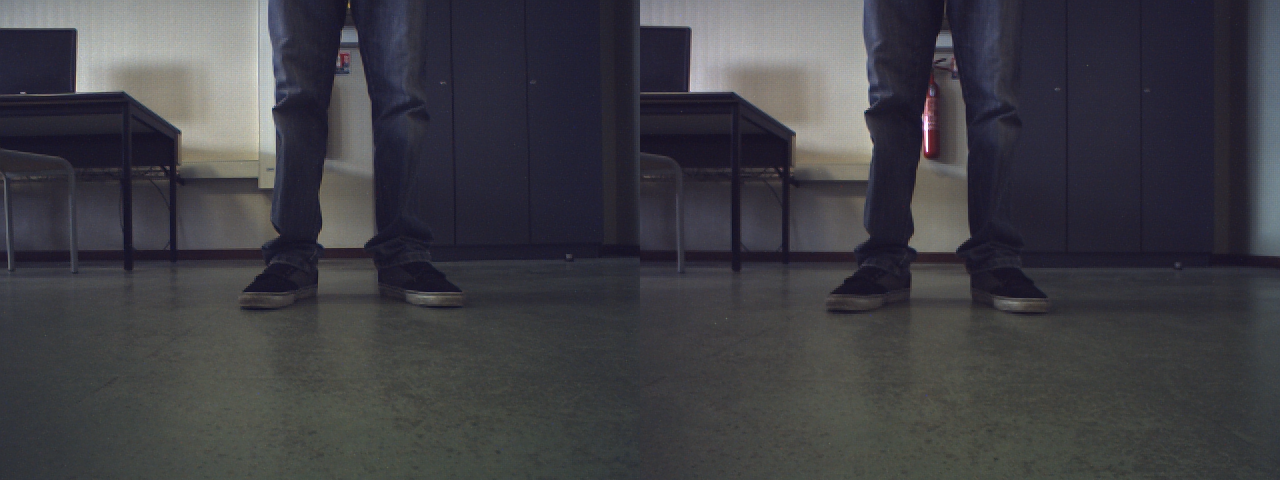
\includegraphics[scale=0.32]{img_0.png}\\
		Figure 4.1.1 Image stéréoscopique de test.
\end{center}

\begin{center}
\begin{tabular}{cc}
  \vspace{0pt} 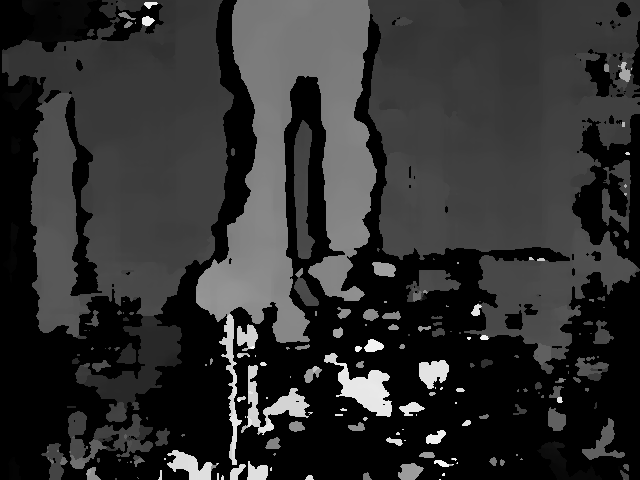
\includegraphics[width=0.49\textwidth]{Carte_de_disparite.png} &
  \vspace{0pt} 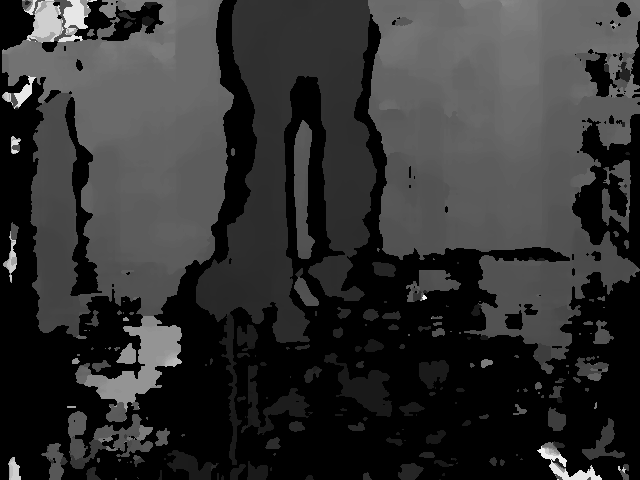
\includegraphics[width=0.49\textwidth]{Carte_de_profondeur.png} \\
    
	Figure 4.1.2 Carte de disparité & Figure 4.1.3 Carte de profondeur
\end{tabular}
\end{center}

Pour tester notre implémentation, nous avons pris des photos issues des caméras du robot. La figure 4.1.1 est l'une d'entre elle. Puis nous avons créé une carte de disparité et une carte de profondeur. 

\section{Faire bouger le robot}
Il faut à présent utiliser la carte de profondeur pour permettre au robot de prendre une décision. Pour cela, nous avons décider de découper la carte de disparité en trois parties verticalement. Nous calculons ensuite la moyenne de chaque partie. Nous choisissons ensuite la moyenne la plus petite, et le robot se dirige dans cette direction. Si il faut aller à gauche ou à droite, le robot s'arrête et tourne dans la direction voulue. Si il faut aller tout droit le robot arrête de tourner et avance.\\

Dans la carte de profondeur (figure 4.1.3), chaque pixel représente une distance. Plus la distance est importante plus la valeur du pixel est élevée et donc plus il sera blanc. Dans le cas contraire, plus la distance est proche, plus la valeur du pixel est basse et donc plus le pixel apparaitra sombre.\\
On peut par exemple voir que dans la figure 4.1.3, les jambes sont plus proches que le mur en arrière plan ; elles sont donc plus sombres.\\
Il faut noter que lorsqu'on affiche une carte de profondeur, le gradient de gris est entre les valeurs 0 et 1 inclus. Cependant, dans nos cartes de profondeur les valeurs peuvent aller jusqu'à 20, distance que nous considérons infinie.

\paragraph{Problèmes rencontrés}
Cette méthode possède comme défaut d'être très imprécise. Si une personne passe devant les objectifs, le robot aura des difficultés à garder sa trajectoire. Le robot ne s'oriente pas tout à fait correctement non plus.

\begin{comment} %Meh
\paragraph{Solutions envisagé}
Pour suivre les trajectoires, le même raisonnement a été proposé mais de manière vertical. C'est à dire que nous découpons la carte de profondeur en trois bandes égales puis nous faisons leur moyenne. Si la bande de gauche à une moyenne plus faible que celle du centre, cela veut dire que la personne à suivre c'est déplacée vers la gauche et donc il suffit de faire tourner le robot jusqu'à ce que la bande du milieu récupère une moyenne plus basse. On applique le même raisonnement sur la bande de droite.\\
\\
\end{comment}


\chapter{Conclusion}

Pour conclure, les objectifs fixés par le cahier des charges ont presque tous été atteinds. Durant la majorité du temps, nous avons travaillé sur la simulation mais nous n'avons malheureusement pas eu assez de temps pour pouvoir tester l'implémentation sur le robot. De plus Unity ne prend pas en charge les unités de distances donc la simulation ne  nous permet pas de dire si le robot fonctionnera correctement.\\
Il reste cependant encore des problèmes à résoudre. Premièrement, la difficulté de définir des paramètres pour le calcul de la carte de disparité font que le programme est sensible aux fluctuations de luminosité. Une solution apportée serait de trouver dynamiquement des paramètres. Enfin, avec l'implémentation actuelle et le fait que faute de temps le programme n'a pas été testé dans des conditions réelles, il est difficile de dire comment il se comportera dans ces conditions. Et donc nous ne pouvons pas certifier que le robot suivra la bonne cible si une autre passe devant les objectifs. Dans le futur certaines perspectives d'amélioration pourraient donc être faite.

\end{document}
